\section{Speicher}
\label{sec:speicher}

\textbf{Begriffe}:
\begin{items}
	\item \underline{Hauptspeicher}: "`Gedächtnis"' des Rechners. Beinhaltet Programme und Daten, die jederzeit und sofort (\emph{random access}) zur Verfügung stehen müssen
	\begin{figure}[H]\centering\label{Hauptspeicher-Struktur}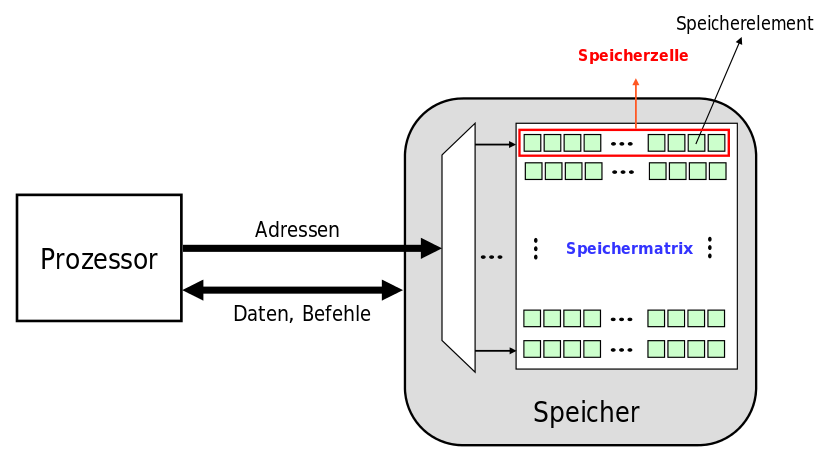
\includegraphics[width=0.33\textwidth]{Hauptspeicher-Struktur}\end{figure}

	\item \underline{Speicherelement}: 1 Bit Speicher

	\item \underline{Speicherzelle}: feste Anzahl von Speicherelementen, auswählbar durch eindeutige Adresse. 8,16,32,\dots Bit

	\item \underline{Speicherwort}: maximale Anzahl an Speicherelementen, die in einem Buszyklus zwischen Mikroprozessor und Speicher übertragen werden können \( \leadsto \) Speicherwortbreite \( = \) \emph{Datenbusbreite}

	\item \underline{Wahlfreier Zugriff}: Jede Speicherzelle kann direkt angesprochen werden (ohne andere Zellen ansprechen zu müssen), Selektion über Adressdecoder

	\item \underline{Speicherorganisation}: Definition über Anzahl \( n \) der Zeilen und Anzahl \( m \) der Speicherelemente pro Zeile, z.B. 16-MBit-DRAM mit Organisation 4Mx4/2Mx8/1Mx16

	\item \underline{Kapazität}: Informationsmenge, die im Speicher untergebracht werden kann (\( n*m \) Bit)

	\item \underline{Arbeitsgeschwindigkeit}:
	\begin{enumeration}
		\item \textbf{Zugriffszeit} (\emph{}access time): maximale Zeit zwischen Anlegen einer Speicheradresse imd Ausgabe der gewünschten Daten

		\item \textbf{Zykluszeit} (\emph{cycle time}): minimale nötige Zeit zwischen zwei hintereinanderfolgenden Adressenaufschaltengen an den Speicher
	\end{enumeration}
\end{items}